\documentclass{beamer}
\usetheme{Singapore}
\usepackage[round,sort]{natbib}
\usepackage{tikz}
\usetikzlibrary{arrows,decorations.pathmorphing,backgrounds,fit,positioning,shapes.symbols,chains}
\usepackage{adjustbox}
\usepackage{verbatim}
\usepackage{graphicx}
\graphicspath{ {etig-05-aiyenggar-images/} }

\title{Firm Effects in Innovation Research}
\subtitle{A Review of Readings}
\author{Ashwin Iyenggar}
\institute[Indian Institute of Management Bangalore] 
{
  Corporate Strategy and Policy\\
  Indian Institute of Management Bangalore
}
\date{11 February, 2017}
\subject{Review of Assigned Readings on Antecedents and Consequences of Firm Effects in Innovation}

% \pgfdeclareimage[height=0.5cm]{university-logo}{university-logo-filename}
% \logo{\pgfuseimage{university-logo}}

\AtBeginSubsection[]
{
  \begin{frame}<beamer>{Outline}
    \tableofcontents[currentsection,currentsubsection]
  \end{frame}
}

\begin{document}

\begin{frame}
  \titlepage
\end{frame}

\begin{frame}{Outline}
  \tableofcontents
  % You might wish to add the option [pausesections]
\end{frame}

\section{Overview}
\begin{frame}{Firm Effects in Innovation Research}{}
\begin{itemize}
\item{Antecedents}
\item{Consequences}
\end{itemize}
\end{frame}

\begin{frame}{Diffusion of Innovation}{}
\begin{itemize}
\item{\cite{Cohen2010} - Technological diffusion from demand and supply side, at different levels of analysis}
\item{\cite{Teece1986} - Empirical study on organizational impediments to adoption of technology}
\item{\cite{Agrawal2014} - Empirical study of peer effects in technology diffusion}
\item{\cite{igami2015} - Empirical study of peer effects in technology diffusion}
\end{itemize}
\end{frame}



\section{\cite{Cohen2010}}
\begin{frame}{The Diffusion of New Technology}{Agenda}
\begin{itemize}
\item{Scope of Definition of Technology Diffusion}
\item{Demand and Supply Side}
\item{Diffusion at different levels of aggregation - worldwide, industry, household}
\end{itemize}
\end{frame}



\section{\cite{Teece1986}}
\begin{frame}{Organizational Barriers to Technology Adoption}{Summary}
\begin{itemize}
\item{Firms take long to adapt to new technology}
\item{Misalignment of incentives may be a major barrier in technological adoption}
\end{itemize}
\end{frame}



\section{\cite{Agrawal2014}}
\begin{frame}{Peer Effects in Technology Diffusion}{Summary}
\begin{itemize}
\item{Is there a causal social interaction effect for the social spillovers to exist?}
\item{The canonical Bass (1969) model assumes social contagion to be a driving force behind accelerating adoption rates}
\item{This article documents and estimates the magnitude of peer effects in diffusion of solar photovoltaic panels}
\item{Issues in indentification of peer effects: endogenous group formation leading to self-selection of peers, correlated unobservables, and simultaneity}
\item{Using daily adoption data, leveraging a DiD to avoid functional or distributional assumptions on the data generating process, controlling for endogeneity, and avoiding the fixed effects biases}
\end{itemize}
\end{frame}



\section{\cite{igami2015}}
\begin{frame}{Peer Effects in Technology Diffusion}{Summary}
\begin{itemize}
\item{Is there a causal social interaction effect for the social spillovers to exist?}
\item{The canonical Bass (1969) model assumes social contagion to be a driving force behind accelerating adoption rates}
\item{This article documents and estimates the magnitude of peer effects in diffusion of solar photovoltaic panels}
\item{Issues in indentification of peer effects: endogenous group formation leading to self-selection of peers, correlated unobservables, and simultaneity}
\item{Using daily adoption data, leveraging a DiD to avoid functional or distributional assumptions on the data generating process, controlling for endogeneity, and avoiding the fixed effects biases}
\end{itemize}
\end{frame}

\bibliography{/Users/aiyenggar/OneDrive/code/bibliography/ae,/Users/aiyenggar/OneDrive/code/bibliography/fj,/Users/aiyenggar/OneDrive/code/bibliography/ko,/Users/aiyenggar/OneDrive/code/bibliography/pt,/Users/aiyenggar/OneDrive/code/bibliography/uz}
\bibliographystyle{apalike}

\end{document}

\begin{comment}
\begin{figure}[h]
\begin{centering}
  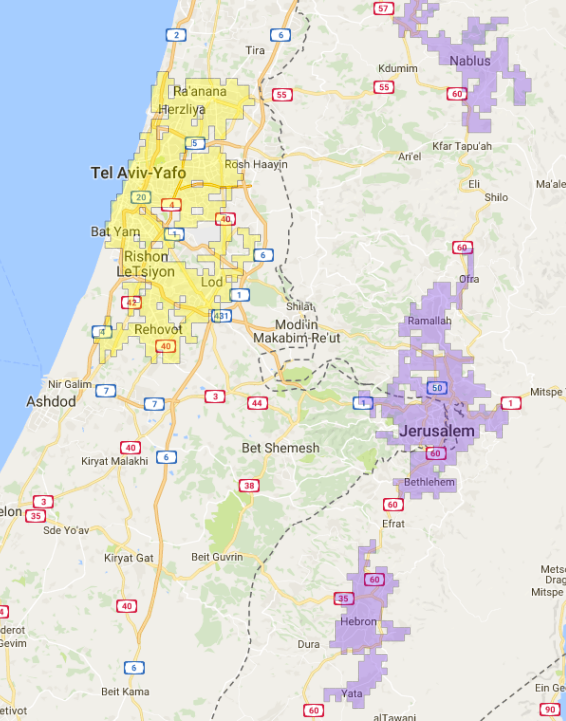
\includegraphics[width=\textwidth]{TelAviv}
  \caption{Geographic Definition of Tel Aviv-Yafo}
   \label{fig:TelAviv}
\end{centering}
\end{figure}
\end{comment}

